\section{EP-Compare}\label{ep-compare}

The EP-Compare program is intended to be used to compare the tabular results of several simulations including the ABUPS summary report. To generate tabular reports in EnergyPlus use the Output:Table:SummaryReports object and make sure the OutputControl:Table:Style includes HTML output. EP-Compare displays bar graphs and monthly line graphs for most of the tabular reports. It can be used in Windows, Linux and Macintosh systems. The main screen is shown below:

\begin{figure}[hbtp] % fig 56
\centering
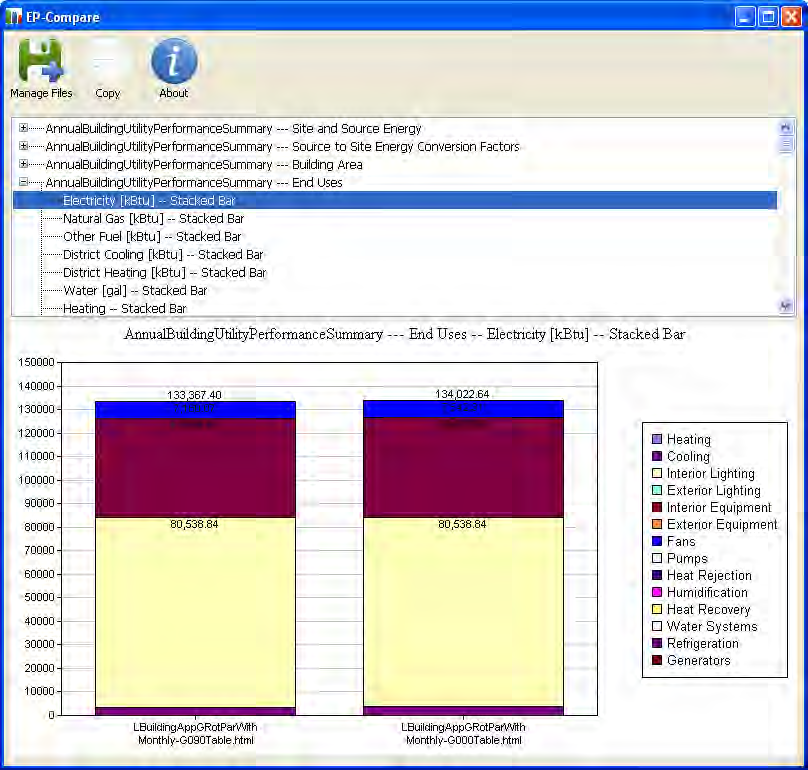
\includegraphics[width=0.9\textwidth, height=0.9\textheight, keepaspectratio=true]{media/image122.png}
\caption{EP-Compare Main Screen \protect \label{fig:ep-compare-main-screen}}
\end{figure}

The main screen shows both the graph being displayed at the bottom and allows the user to select a graph from a list at the top. The list of graphs is based on each table name and subtable name and then has a list of graphs supported including stacked bars, simple bar, 100\% stacked bars, side-by-side bars, and monthly line graphs. The program window can be resized.

The first time the program is started no graphs are shown because no files have been selected. To select files use the ``Manage Files'' button. This brings up the Manage Files dialog box shown below:

\begin{figure}[hbtp] % fig 57
\centering
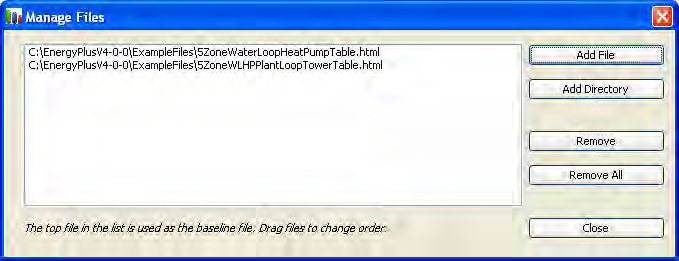
\includegraphics[width=0.9\textwidth, height=0.9\textheight, keepaspectratio=true]{media/image123.png}
\caption{EP-Compare Dialog box \protect \label{fig:ep-compare-dialog-box}}
\end{figure}

This dialog lets you add and remove files from the list of files. The files selected should be HTML or HTM files that are produced by EnergyPlus when using the Output:Table:SummaryReports object with OutputControl:Table:Style set to produce HTML files. It is best to compare files that have similar reports otherwise missing values will be shown as zeros.The dialog also provides a button to add entire directories of files but that adding too many files makes the graphs difficult to understand. To change the order that files appear in the graph, the files can be dragged up and down the list of files in the Manage Files dialog. The dialog box window can be resized to view longer files names if necessary.

When EP-Compare is started again, the files last selected are shown in the graph if they are still available.

The Copy button allows the current graph (as it is sized in the window) to be copied to another application such as Microsoft Word or PowerPoint. To paste a copied image to those programs use the Paste Special option and select one of the bitmap formats.
